\documentclass[text.tex]{subfiles}

\begin{document}

\section{Delone set and Voronoi tessellation}

This section provides the definitions of a Delone set a covering radius and a Voronoi tessellation.

\begin{definition}
\label{def:Delone}
Let $P\subset \mathbb{R}^n$ and let there exist $R>0$ and $ r>0$ such that:
$$\forall x,y\in P,\, x\neq y: r\leq \|x-y\|$$
$$\forall z\in\mathbb{R}^n\; \exists x\in P: \|z-x\|\leq R$$
Then $P$ is called \textbf{Delone} set.\\
For each Delone set $P$ \textbf{covering radius} is defined as:
$$R_c = \inf\{R>0\,|\, \forall z\in\mathbb{R}^n \exists x\in P: \|z-x\|\leq R\}$$
\end{definition}

\begin{definition}
Let $P\subset \mathbb{R}^n$, $P$ is a discrete set and $x\in P$. Then
$$V(x) = \left\{ y \in \mathbb{R}^n \,|\, \forall z \in P, z\neq x:\, \|y-x\|\leq\|y-z\| \right\}$$
is called \textbf{Voronoi polygon} of $x$ on $P$.

Voronoi polygon $V(x)$ is said to belong to the point $x$ and $x$ is called the center of the polygon $V(x)$. The subset of $P$ that directly shapes the polygon $V(x)$ is called the domain of the polygon.
\end{definition}

\begin{remark}
Example of a Delone set with the Voronoi tessellation can be seen in Figure \ref{fig:finiteSectionQuasi}.
\end{remark}

\begin{theorem}
\label{the:radiusLimit}
Let $P\subset \mathbb{R}^n$ be a Delone set and $R_c$ its covering radius. For any $x\in P$ define:
$$N_x = \{z\in P\,|\, z\neq x \wedge \|z-x\|\leq 2R_c\}$$
Then Voronoi tile of $x$ on $P$ is
$$V(x) = \bigcap_{z\in N_x} \left\{ y \in \mathbb{R}^n \,|\, \|y-x\|<\|y-z\| \right\}$$
\end{theorem}

\begin{remark}
Theorem \ref{the:radiusLimit} gives an algorithm for Voronoi polygon construction. First it limits the amount of points of $P$ that need to be considered and also it shows that the polygon can be constructed by series of cuts between the center and each of the points form $N_x$. 
\end{remark}
%
\clearpage
\section{Two-dimensional quasicrystals}%=======================================================================================================================
\label{sec:twoDimension}
In the following section a two-dimensional quasicrystal is defined and analyzed. Thanks to the Theorem \ref{the:twoToOne}, analysis of one-dimensional quasicrystals can be in some way applied to the two-dimensional quasicrystals as well. 
\begin{definition}
Vectors $\alpha_1$, $\alpha_2$, $\alpha_3$ and the set $M$ denote the following.
$$\alpha_1 = \left( 1,0 \right) \quad \alpha_2 = \left( \frac{2-\beta}{2}, \frac{1}{2} \right) \quad \alpha_3 = \left( \frac{\beta-2}{2}, \frac{1}{2} \right)$$
$$M = \ring\alpha_1 + \ring\alpha_2$$
\end{definition}

\begin{figure}[h]
\centering
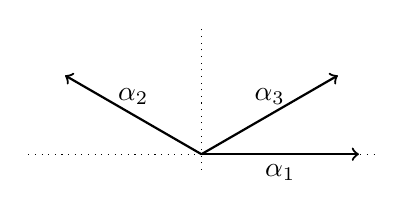
\begin{tikzpicture}[scale=2]
\draw [dotted] (0,-0.1) -- (0,0.8);
\draw [dotted] (-1.1,0) -- (1.1,0);

\draw [thick,->] (0,0) -- node[below] {$\alpha_1$} (1,0);
\draw [thick,->] (0,0) -- node[above] {$\alpha_2$} (-0.866,0.5);
\draw [thick,->] (0,0) -- node[above] {$\alpha_3$} (0.866,0.5);
\end{tikzpicture}
\caption{Plot of the three vectors $\alpha_1$, $\alpha_2$ and $\alpha_3$.}
\end{figure}

\begin{remark}
The vectors and the set from previous definition are key to two-dimensional quasicrystal definition. The set $M$ is used as a two-dimensional equivalent to $\ring$ from the one-dimensional quasicrystal. Function from following definition is used as a two-dimensional equivalent to $'$.
\end{remark}

\begin{definition}
\label{def:starFunction}
Function $\ast: M \to M$ is called \textbf{star} function:
$$v^\ast = (a\alpha_1 + b\alpha_2)^\ast = a'\alpha_1 + b'\alpha_3 \quad\forall a,b\in\ring$$
\end{definition}

\begin{remark}
Simple consequence of Definition \ref{def:starFunction} is that $\alpha_1^\ast = \alpha_1$ and $\alpha_2^\ast = \alpha_3$.
\end{remark}

\begin{definition}
Let $\Omega \subset \mathbb{R}^2$ be bounded set with nonempty interior. Then \textbf{two-dimensional quasicrystal} with the window $\Omega$ is defined as:
$$\quasi{\Omega} = \left\{ x \in M\,|\,x^\ast \in \Omega \right\}$$
\end{definition}

\begin{remark}
$\quasi{\Omega}$ where $\Omega \subset \mathbb{R}^2$ always denotes two-dimensional quasicrystal.
\end{remark}

\begin{remark}
\label{rem:quasiProperties}
The same properties from Theorem \ref{the:quasiProperties} for the one-dimensional quasicrystals apply to the two-dimensional quasicrystals as well.
\end{remark}

To analyze the two-dimensional quasicrystals again only windows of a certain shape will be considered. That is sufficient because of Remark \ref{rem:quasiProperties}. The chosen window shape is a rhombus. 

\begin{theorem}
\label{the:twoToOne}
Let $I = [c,d)$, then for the rhombus $\Omega = I\alpha_1^\ast + I\alpha_2^\ast$ and the quasicrystal $\quasi{\Omega}$ it holds that: 
$$\quasi{\Omega} = \quasi{I}\alpha_1 + \quasi{I}\alpha_2$$
The size of the rhombus refers to the size of the interval $|I|$ also a base rhombic window refers to a rhombic window constructed from a base window $I$.
\end{theorem}

\begin{figure}[h]
\centering
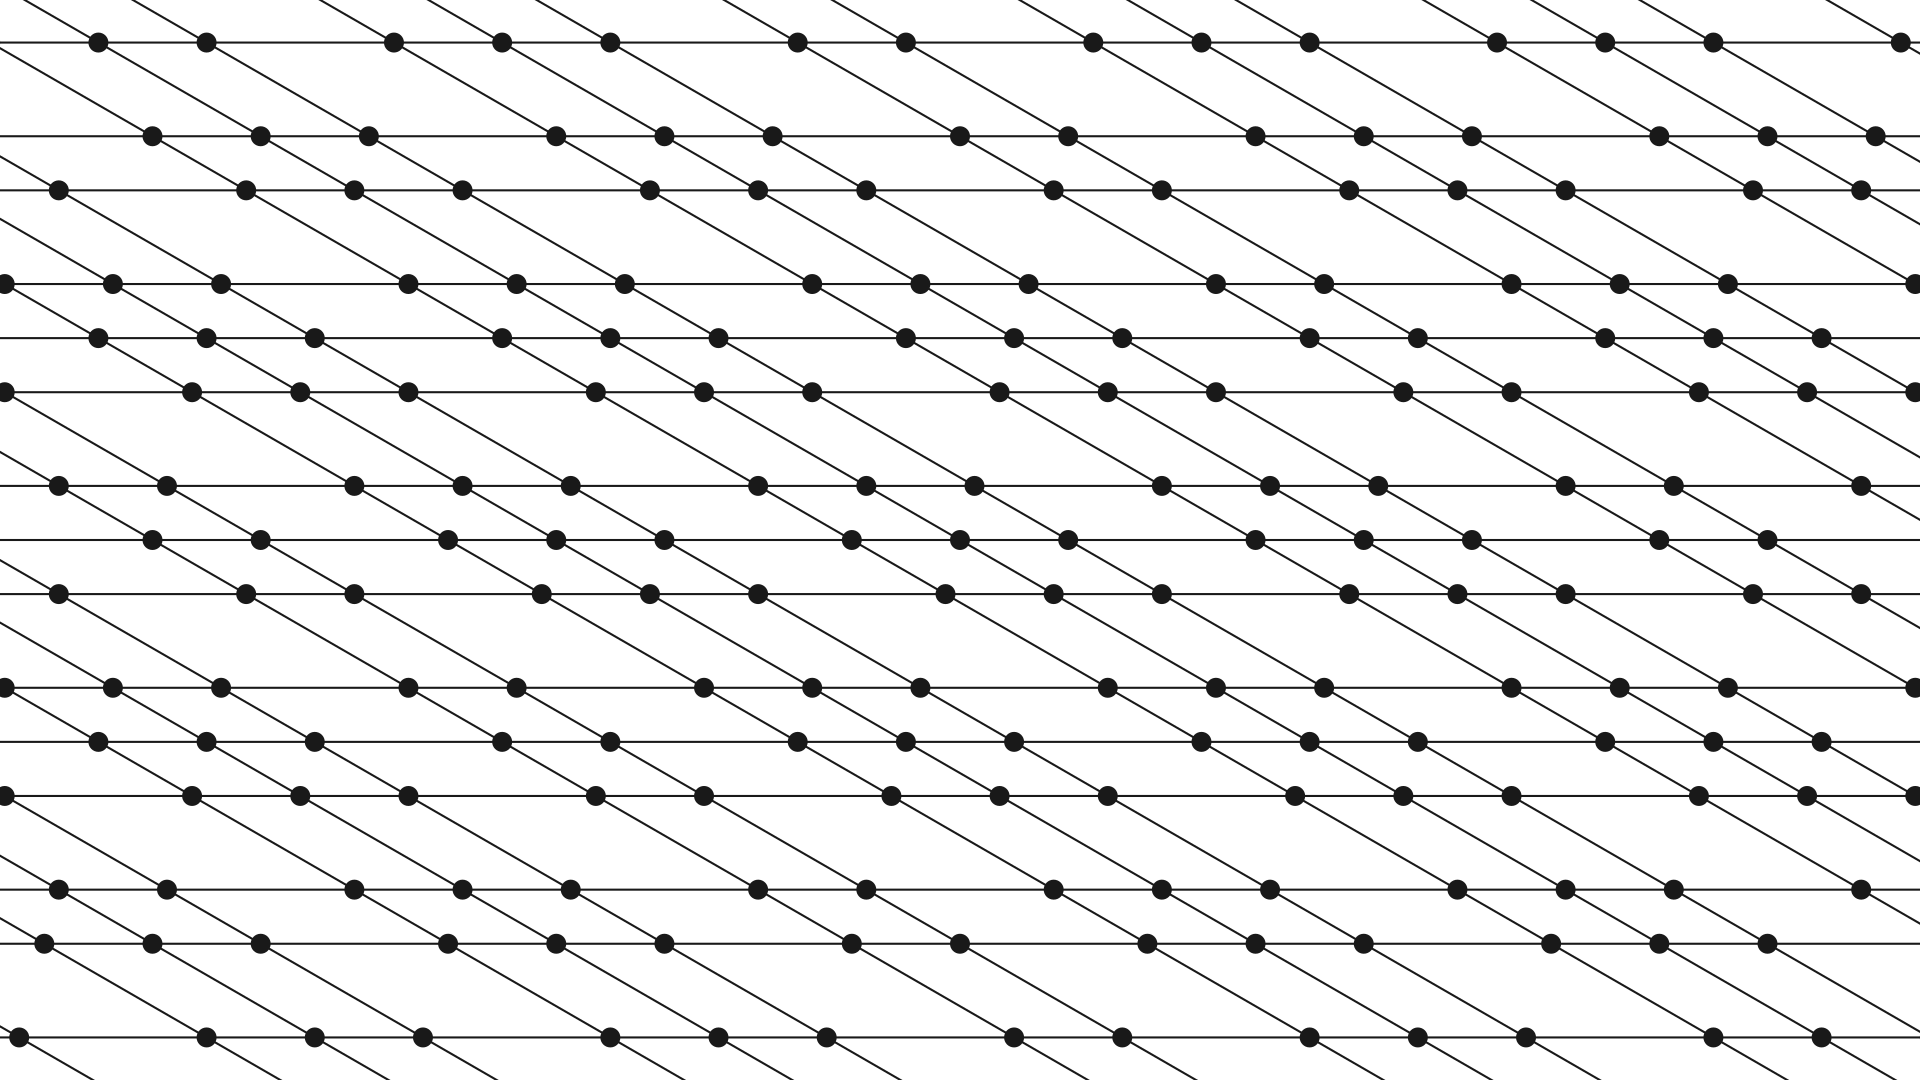
\includegraphics[width=\textwidth]{rhombus_construction}
\caption{Illustration of the construction of the two-dimensional quasicrystal with a rhombic window from two one-dimensional quasicrystals. Horizontal lines mark copies of $\quasi{I}\alpha_1$ and the skewed lines mark copies of $\quasi{I}\alpha_2$.}
\label{fig:quasiRhombusConstruction}
\end{figure}

\begin{remark}
Note in the previous theorem that while $\Omega \subset \RN^2$ and so $\quasi{\Omega}$ is a two-dimensional quasicrystal, $I \subset \RN$ and so $\quasi{I}$ is a one-dimensional quasicrystal. Illustration of the construction is in the Figure \ref{fig:quasiRhombusConstruction}.
\end{remark}

From the analysis of one-dimensional quasicrystals and Theorem \ref{the:twoToOne} it follows that the two-dimensional quasicrystals are Delone sets.  

To analyze distribution of the points of a two-dimensional quasicrystal, Voronoi tessellation is used. The goal is to catalog shapes of all Voronoi tiles that appear in a quasicrystal with a rhombic window. 

First an algorithm for generation of a finite section of a quasicrystal is presented. 

%
\clearpage
\section{Generation of a finite section of a quasicrystal with a rhombic window}%=======================================================================================================================
The algorithm is rather simple. It uses the stepping function and Theorem \ref{the:twoToOne}. 

\paragraph{Algorithm definition} The algorithm receives as an input a rhombic window $\Omega = I\alpha_1^\ast + I\alpha_2^\ast$ and bounds $x_1, x_2, y_1, y_2 \in \ring$.
The algorithm returns a subset of the quasicrystal $\quasi{\Omega}$ bounded by the given bounds.
$$\quasi{\Omega}\cap([x_1,x_2]\times[y_1,y_2])$$

First the one-dimensional interval $I = [c,d)$ needs to be scaled and moved in such a way, that it becomes a base window and contains $0$.
$$(\exists k\in\ZN)(\exists \lambda\in\ring) : \left(I = \beta^k\tilde{I}+\lambda\right) \wedge \left(|\tilde{I}| \in \left(\frac{1}{\beta},1\right] \right)\wedge \left(0\in\tilde{I}\right)$$

Now the stepping function can be used to iterate from 0 and generate enough points of the quasicrystal $\quasi{\tilde{I}}$ to cover the bounds. However since the bounds are for the quasicrystal $\quasi{\Omega}$ they need to be transformed to be applicable to the quasicrystal $\quasi{\tilde{I}}$. 
\begin{align*}
\tilde{x_1} &= x_1 & \tilde{y_1} &= 2y_1 \\
\tilde{x_2} &= x_2 + (\beta-2)(y_2-y_1) & \tilde{y_2} &= 2y_2 
\end{align*}
The stepping function is then used to acquire two sections of the quasicrystal $\quasi{\tilde{I}}$: $\quasi{\tilde{I}}\cap[\tilde{x_1},\tilde{x_2}]$ and $\quasi{\tilde{I}}\cap[\tilde{y_1},\tilde{y_2}]$.

Each section needs to be transformed back:
$$\quasi{I} = \beta^{-k}\quasi{\tilde{I}} + \lambda'$$
and finaly the finite section of the quasicrystal $\quasi{\Omega}$ is constructed:
$$\quasi{\Omega} = \quasi{I}\alpha_1 + \quasi{I}\alpha_2$$

\begin{figure}[h]
\centering
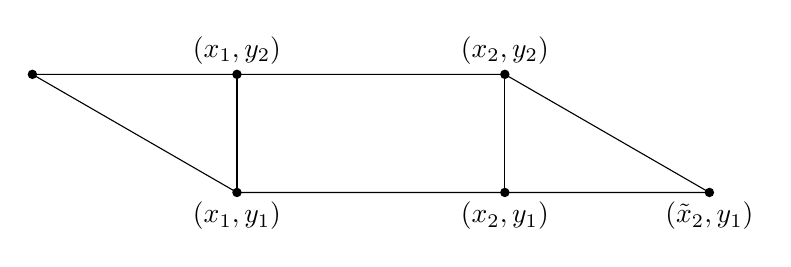
\begin{tikzpicture}[scale=3]
% nodes
\draw [-] (0,0)  -- (-2,0) -- (-2.86602540378,0.5) -- (-0.86602540378,0.5) -- cycle;
\draw [-] (-0.86602540378,0)  -- (-2,0) -- (-2,0.5) -- (-0.86602540378,0.5) -- cycle;

\fill (0,0) circle (0.02);
\fill (-2,0) circle (0.02);
\fill (-2.86602540378,0.5) circle (0.02);
\fill (-0.86602540378,0.5) circle (0.02);
\fill (-0.86602540378,0) circle (0.02);
\fill (-2,0.5) circle (0.02);

\node [below] at (0,0) {$(\tilde{x}_2,y_1)$};
\node [below] at (-0.86602540378,0) {$(x_2,y_1)$};
\node [below] at (-2,0) {$(x_1,y_1)$};
\node [above] at (-0.86602540378,0.5) {$(x_2,y_2)$};
\node [above] at (-2,0.5) {$(x_1,y_2)$};

\end{tikzpicture}
\caption{Illustration of how big parallelogram section of the quasicrystal (not a window) is needed to acquire a rectangular one.}
\label{fig:finiteSectionRhombus}
\end{figure}

\begin{remark}
Due to the way the two-dimensional quasicrystal is constructed, the result will contain more points then requested (Figure \ref{fig:finiteSectionRhombus}). However the excess points can be easily discarded.
\end{remark}

\begin{figure}[h]
\centering
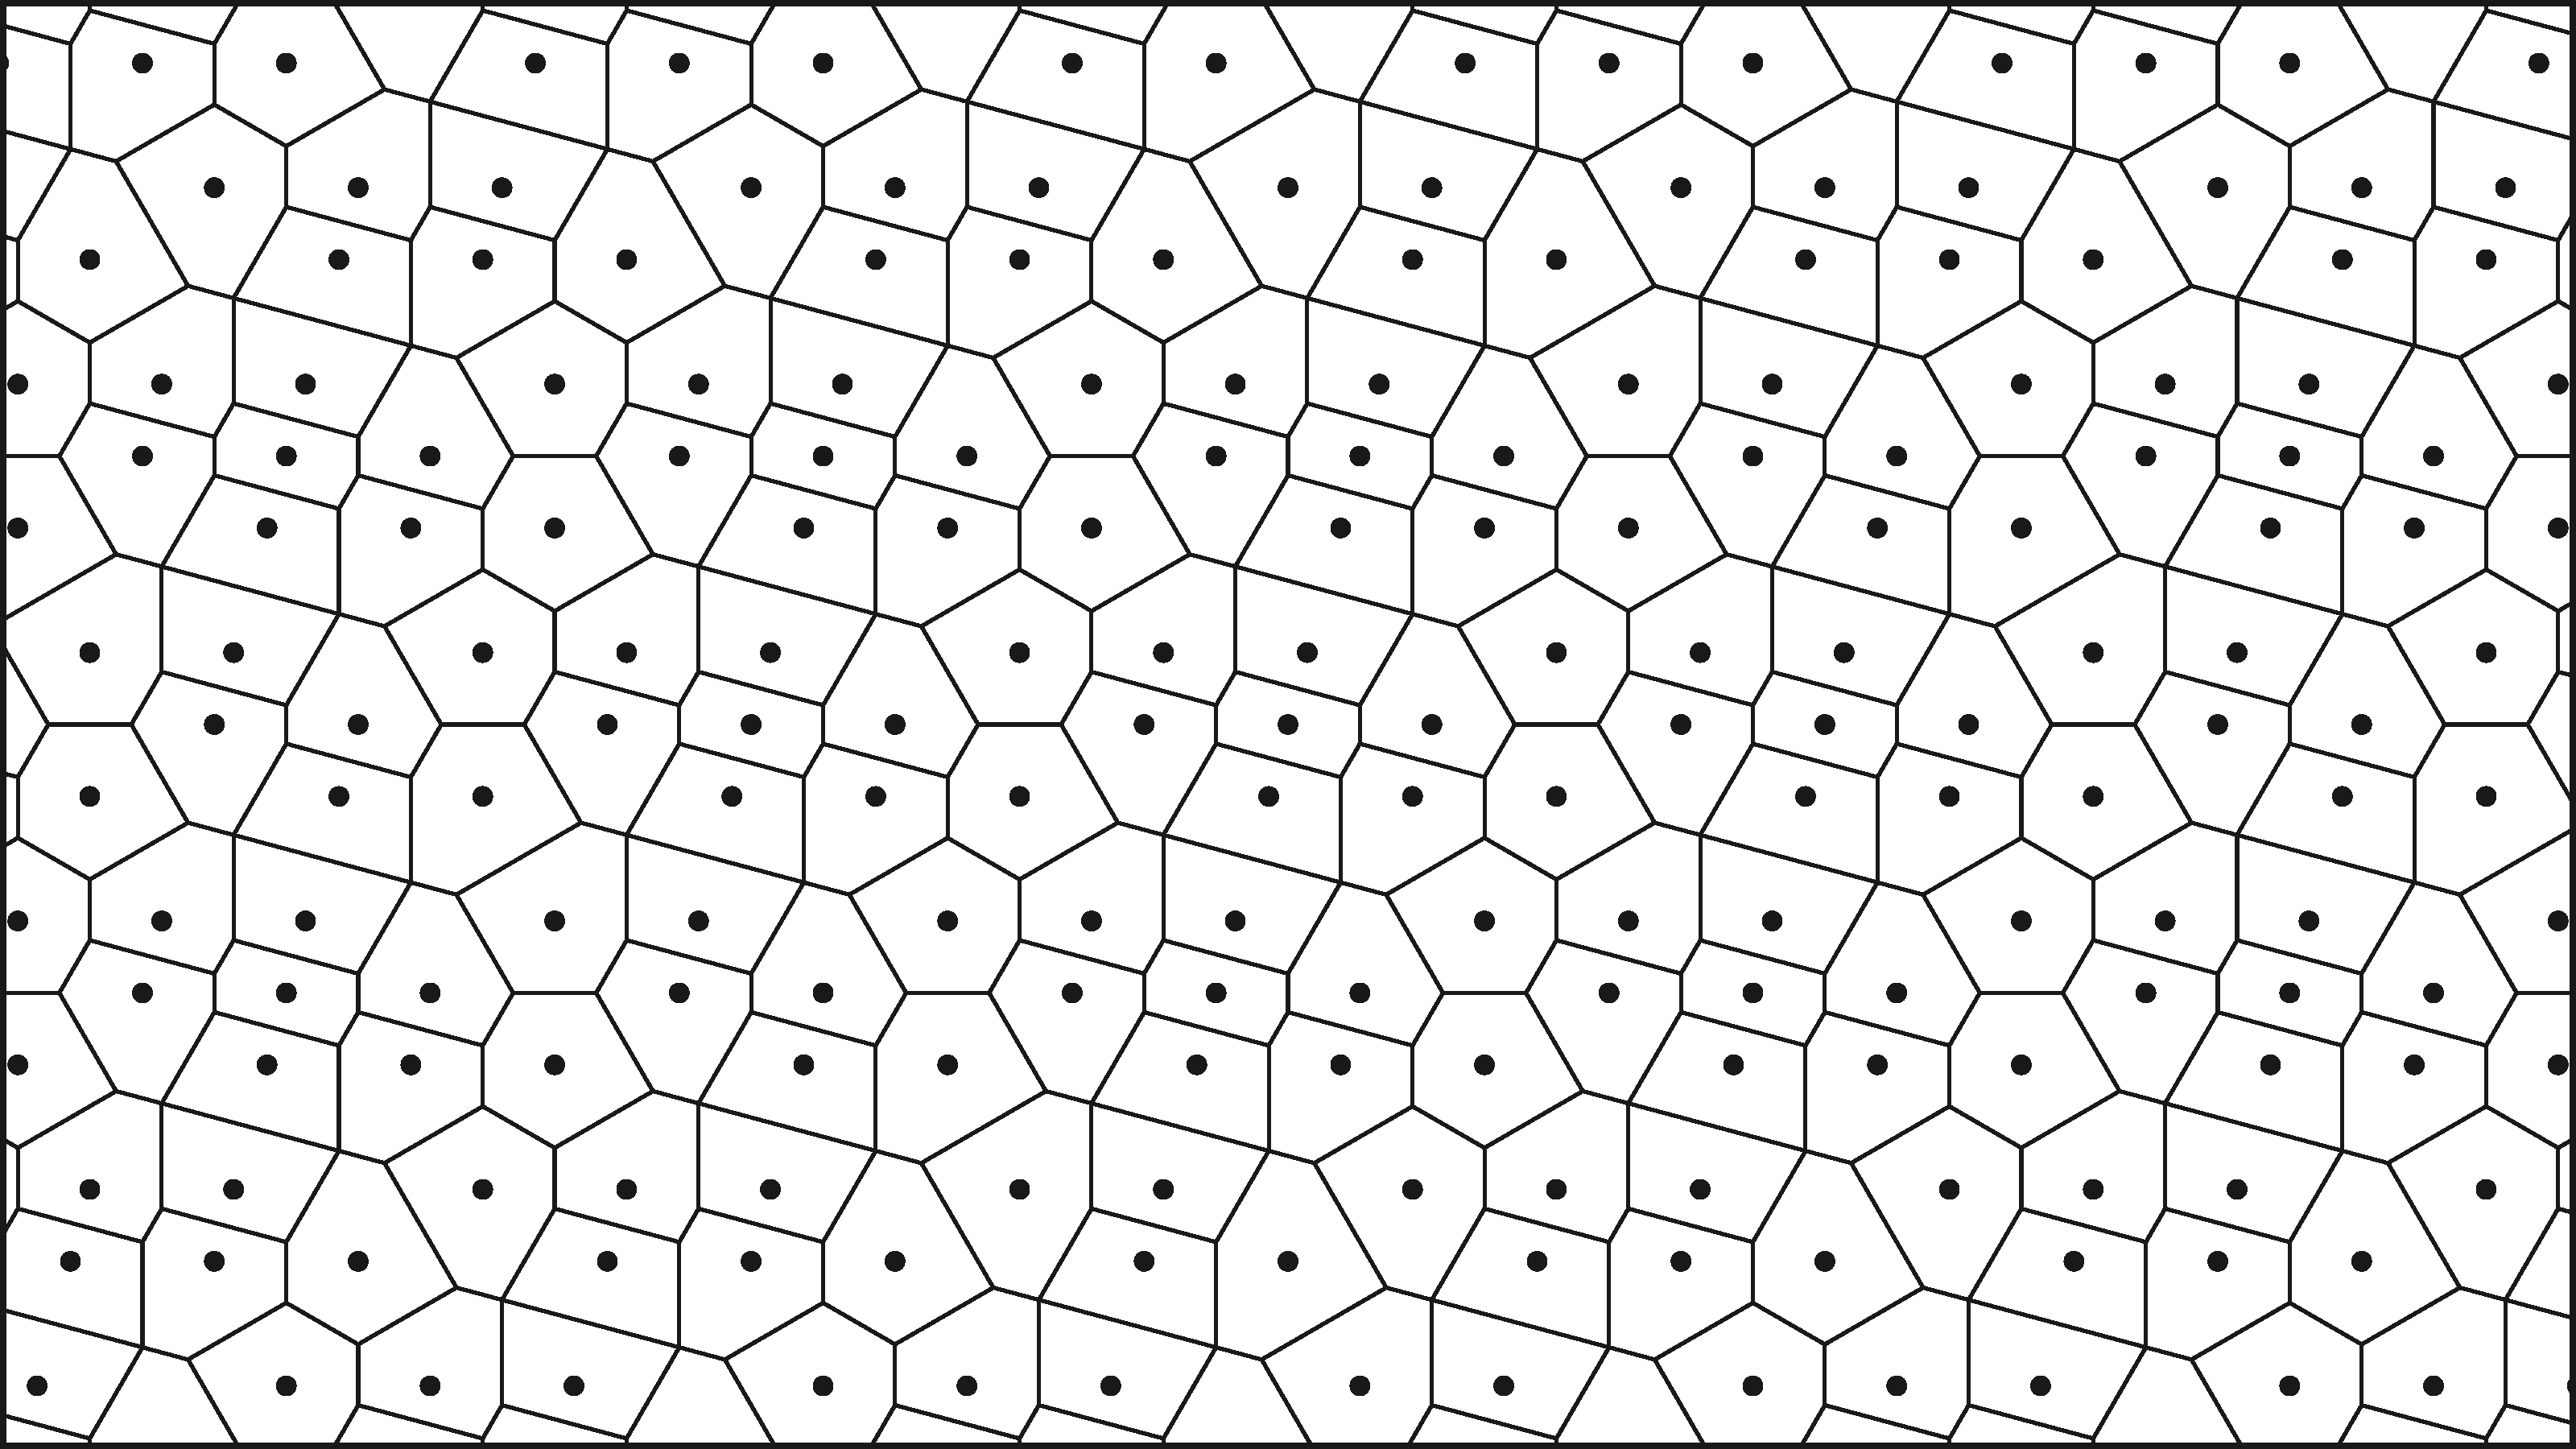
\includegraphics[width=\textwidth]{rhombus_window_01_(-22_6_7)}
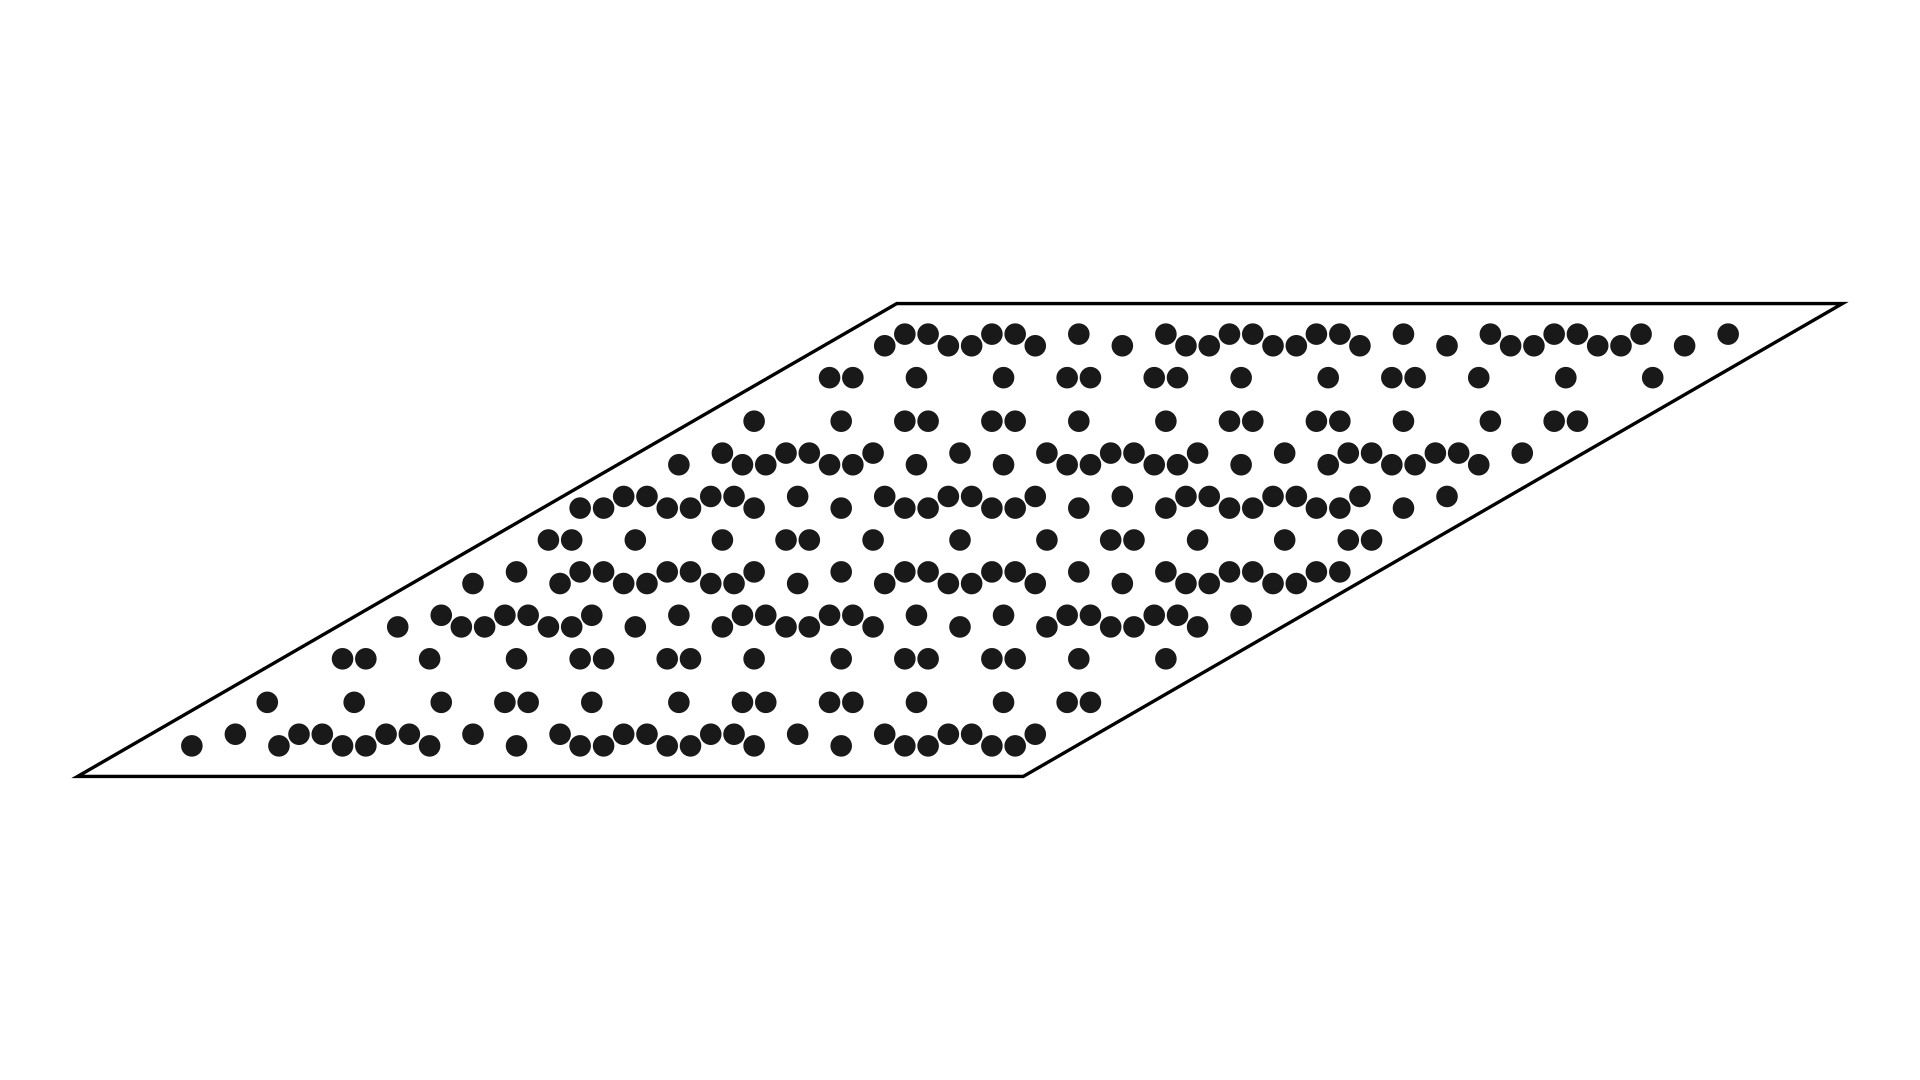
\includegraphics[width=\textwidth]{rhombus_window_01_(-22_6_7)_window}
\caption{Finite section of the quasicrystal $\quasi{I\alpha_1^\ast + I\alpha_2^\ast}$ where $|I| = \frac{6\beta-22}{7}$ with the Voronoi tessellation and the rhombic window $I\alpha_1^\ast + I\alpha_2^\ast$ with $\ast$ images of the points from the finite section.}
\label{fig:finiteSectionQuasi}
\end{figure}

The next goal is now to catalog all different Voronoi polygons that appear in a quasicrystal for a single window. 
\end{document}
